\documentclass{article}
\usepackage[pdftex]{graphicx}
\usepackage{mathtools}
\usepackage{Sweave}
\begin{document}
\Sconcordance{concordance:lab9.tex:lab9.Rnw:%
1 3 1 1 0 3 1 1 2 1 0 1 2 1 0 1 1 3 0 1 2 1 1 1 17 10 1 1 2 4 0 1 2 21 1 1 4 10 %
0 1 2 4 1 1 11 13 0 1 2 15 1}



\begin{Schunk}
\begin{Sinput}
> library(knitr)
> # set global chunk options
> opts_chunk$set(fig.path='figure/minimal-', fig.align='center', fig.show='hold')
> options(formatR.arrow=TRUE,width=90)
\end{Sinput}
\end{Schunk}



\textbf{Abstract}
In the following report we wil preform a basic linear regression to explain how well one data set predicts a corresponding set. In particular, we will reproduce the work done in sections 3.1 of \emph{Simple Linear Regression} using the exact same data sets and producing some of the same graphics.

\textbf{Introduction}
The goal of this paper is to advise retailers on how to spend their advertising money amongst the available media outlets. We will do this by regressing the relative ammount of money spent on advertising on the total sales, determining if there is some relationship, and determine the strength of the relationship. Using this information we can provide statistically supported advise to the retailer.\\
\textbf{Data}
The data in question is the Advertising data set found at \emph{http://www-bcf.usc.edu/~gareth/ISL/Advertising.csv}. The data has a total of 200 observation in four variables: \textbf{Tv}, \textbf{Radio}, \textbf{Newspaper}, and \textbf{Sales}. The \textbf{Sales} data is given in thousands of units, and all other data is given in thousands of dollars spent.\\
\textbf{Methodology}
In this paper we will only consider the \textbf{Tv} data and its influence on \textbf{Sales}. The methods used can easilly be extended to other variables if desired.
To describe the relationship we first consider a basic scatterplot of \textbf{Tv} against \textbf{Sales}: \\
\begin{Schunk}
\begin{Sinput}
> plot(x = Tv, y =  Sales, col = "Red", pch = 16, cex = .75)
\end{Sinput}
\end{Schunk}
\\
There appears to be a linear relationship between \textbf{Tv} and \textbf{Sales}, as \textbf{Tv} increases \textbf{Sales} tends to as well. Thus, we decide on the following linear model:
$$ Y = X*\beta $$ \\
With $Y \coloneqq \bold{Sales}$ and $X \coloneqq \bold{Tv}$. Upon fitting the model to our data we well be able to solve for the optimal $\beta$. Recall that in linear regression the objective function is to minimize the following following L2 norm over all possible $\beta$ values:
$$ \lVert Y - X\beta \rVert_{2} $$
Some basic matrix algebra gives the following optimal value of $\beta$ given some $Y$ and $X$ data matricies:
$$ \hat{\beta}_{OLS} \coloneqq (X^{T}X)^{-1}X^{T}Y $$
Next we consider the Residual Standard Error, or RSE. The RSE is considered a measure of "lack of fit", meaning it measures how poorly a model fits the data. We define RSE as follows:
$$ RSE \coloneqq \sqrt{\dfrac{1}{n-2}\sum_{i=1}^{n} (Y_{i} - \hat{Y}_{i})} $$
Thus, we may think of RSE as the average deviation from the OLS prediction.\\
We will also consider the $R^{2}$ statistic to help determine the strength of the correlation between our variables, $R^{2}$ is given by:
$$ R^{2} \coloneqq \dfrac{TSS - RSS}{TSS} = 1 - \dfrac{RSS}{TSS} $$
$$ RSS \coloneqq \sum_{i=1}^{n} (Y_{i} - \hat{Y}_{i})^{2} $$
$$ TSS \coloneqq \sum_{i=1}^{n} (Y_{i} - \bar{Y})^{2} $$
Thus, we may think of $R^{2}$ as a proportion of explained variance : total variance.\\
Finally we consider the F-statistic, which can be used to determine if our model has excess regressors. The F test uses the following hypothesis:
$$ H_{0} : \beta = 0$$
$$ H_{1} : \beta \neq 0$$

\textbf{Results}
Once we loaded and prepared the data we observed the following values relating to $\hat{\beta}$ in Table 1:

\begin{table}[ht]
\centering
\begin{tabular}{rrrrr}
  \hline
 & Estimate & Std. Error & t value & Pr($>$$|$t$|$) \\ 
  \hline
(Intercept) & 7.0326 & 0.4578 & 15.36 & 0.0000 \\ 
  Tv & 0.0475 & 0.0027 & 17.67 & 0.0000 \\ 
   \hline
\end{tabular}
\caption{Regressor Analytics} 
\end{table}and recorded statistics relating to the overall model in Table 2 on the following page.\\
We note that Pr(>|t|) is so small that it is rounded down to 0, implying the \textbf{intercept} and \textbf{Tv} regressors both contribute significantly in the prediction of \textbf{Sales}, which in turn tells us to keep both in the model. To further support this we note the large t-scores for each regressor, implying they are significant to the model.\\
Next we look at the actual values and interpret them. The intercept ($\hat{\beta}_{0}$) is 7.0326, this can be interpreted as the total \textbf{Sales} if no money is spent on \textbf{Tv}. The Tv value ($\hat{\beta}_{1}$) is .0475, this can be interpreted as the unit of \textbf{Sales} increase per one unit increase in \textbf{Tv}. Note Table 1 also provides standard errors, allowing us to (if we wish) produce ($100 * \alpha$) \% confidence intervals of the form:
$$ \hat{\beta}_{i} \pm t_{n-2}(\dfrac{\alpha}{2})* Std.\ Error_{i} $$\\
Now we consider the information in Table 2.
\begin{table}[ht]
\centering
\begin{tabular}{rlr}
  \hline
 & Statistics & Values \\ 
  \hline
1 & RSS & 2102.53 \\ 
  2 & MSE & 10.51 \\ 
  3 & RSE & 3.26 \\ 
  4 & R2 & 0.61 \\ 
  5 & FStat & 312.14 \\ 
   \hline
\end{tabular}
\caption{Model Analytics} 
\end{table}
The RSS gave a value of 2102.53, which is not too helpful in judging the models performance. The MSE was only 10.51, which has a direct interpretation as the average of the squares of the errors given by our model.\\
The RSE gave a value of 3.26, as described in the \textbf{Methodology} section this is interpreted as a measure of 'lack of fit'. A relatively small RSE, like 3.26, implies that our model is fitting the data relatively well.\\
The $R^{2}$ statistic is described in the \textbf{Methodology} section as well. Noting that the value is .61 for this particular model, it is safe to say \textbf{Tv} has a positive correlation with \textbf{Sales}, albeit not a perfect correlation but a clear correlation none the les.\\
Recall the FStat tells us the probability our model contains excess regressors. In our model the we have an F-Statistic with (1, 198) degrees of freedom and a value of 312.14. Using this information we can use the F-Statistic table (an online tool can be found here: \emph{http://stattrek.com/online-calculator/f-distribution.aspx}) to see that we would reject $$H_{0}\ \forall \ \alpha > 1.525879e-05$$

\textbf{Conclusions}
Using the information discussed in \textbf{Results} and \textbf{Methodology}, we have sufficient evidence to support the conclusion that spending more money on \textbf{Tv} results in an increase in \textbf{Sales}.\\
By viewing the scatterplot shown in Figure 1 with the Least Squares line superimposed on it we can clearly see that this claim holds:
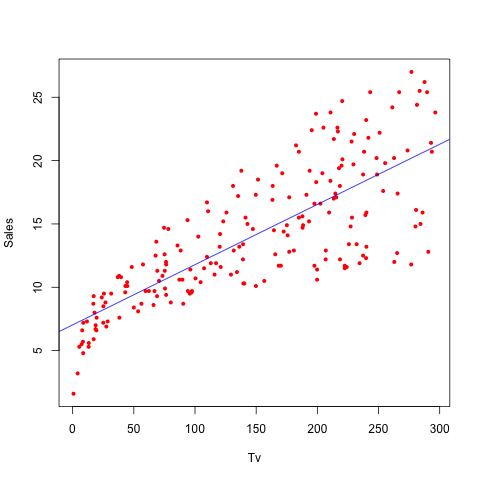
\includegraphics{images/scatterplot-tv-sales.png}
In conclusion, we advise retailers to use the following equation to estimate \textbf{Sales}:
\textbf{Sales} = 7.0326 + .0475*\textbf{Tv} \\
To further elaborate, we expect a increase of .0475 thousand units sold for every 1 thousand dollars spend on Tv advertising. Note these results were calculated without considering any kinds of external influences, one off events, or other regressors.\\
Similarly, we would advise retailers to be aware of the RSE. The RSE is informing us that, on average, our predictions for \textbf{Sales} are 3.26 thousand units sold off their true value.

\end{document}
